% Provenance (never printed): see sources/outline_sources.md (Year 2: mid-latitude cyclones and
% fronts; jets and Rossby waves, descriptive; tropical cyclones; numerical weather prediction,
% principle). Definitions after the NWS glossary and UCAR; cyclogenesis conditions after the NOAA
% AOML FAQ; potential intensity after Gilford (2021, pyPI); conveyor belts after Raveh-Rubin and
% Catto (2019); blocking after Wang and others (2026); predictability after Krishnamurthy (2019),
% Selz and others (2022) and ECMWF. The Lorenz system from figdata/bachelor-2/weather.py; the
% fronts, waves and storms of the examples, exercises and problem are invented, their values
% computed in the Book 4 scratch calculator calc/ch22.py.
\chapter{天气系统}\label{ch:b2:weather-systems}

如今，四天后的预报准确度已与三十年前一天后的预报相当，
每十年左右，有效预报的时长便增加约一天。但是，
对某一天、某一地点天气的预报，超过十天便不再可靠，而仅靠更好的计算机
也无法把这一极限推得很远：大气会放大自身的微小不确定性。
本章介绍预报所关注的天气系统，包括中纬度的锋与低压，
急流中的波动与热带气旋，然后讲它们如何被预报，
以及预报为何必定要在某处停止。
% ledger: mo:accuracy, bauer:day-per-decade, krish19:predictability

\begin{recall}
\textbf{来自中小学分册}：气团、锋、冷锋与暖锋、低压与
反气旋、等压线与天气预报；热带气旋、其风暴眼与眼墙、
萨菲尔–辛普森等级。\textbf{来自本科一年级分册}：气压梯度力、
科里奥利参数 $f = 2\Omega\sin\varphi$、地转平衡、气旋与反气旋、
三个环流圈、西风带与急流。\textbf{来自物理各册}：热机
及卡诺循环的效率。\textbf{来自\cref{ch:b2:atmospheric-thermodynamics}}：
饱和、\omterm{def:b2:atmospheric-thermodynamics:moist-adiabat}{湿绝热线}、$\theta_e$、\omterm{def:b2:atmospheric-thermodynamics:instability}{条件不稳定}与 CAPE。
\end{recall}

\section{锋}\label{sec:b2:weather-systems:fronts}

中小学分册把锋画成地图上的线。锋是两个气团之间倾斜的分界面与地面相交的线，
其天气即来自这一倾斜。

\begin{definition}[锋面；准静止锋；锢囚锋]\label{def:b2:weather-systems:fronts}
锋的\emph{锋面}\index{锋面}是两个气团之间倾斜的分界面，
两者中较重、较冷的一个位于下方，呈楔形；地图上的锋即其
与地面的交线。\emph{准静止锋}\index{准静止锋}是指
移动非常缓慢或几乎不动的锋。\emph{锢囚锋}\index{锢囚锋}是
由两个锋复合而成，当冷锋追上暖锋或准静止锋时形成。
\end{definition}
% ledger: nws4:front, nws4:stationary, nws4:occluded

当两个气团都无法推动对方时形成\omterm{def:b2:weather-systems:fronts}{准静止锋}，此时风沿锋
吹而非穿过锋；它可停留数日，多云且有雨，然后再以冷锋
或暖锋的形式重新移动。地图上，它交替画出朝向暖空气的冷锋蓝色三角形，
与朝向冷空气的暖锋红色半圆形相间。\omterm{def:b2:weather-systems:fronts}{锢囚锋}以紫色绘制，两种符号画在同一侧。
\omterm{def:b2:weather-systems:fronts}{锢囚锋}以紫色绘制，两种符号画在同一侧。冷锋之后的气团
较冷时，冷锋滑入暖锋之下，将其抬离地面，称为冷式锢囚；当暖锋之前的气团
较冷时，冷锋则爬升到暖锋之上，称为暖式锢囚。
% ledger: ucar4:stationary-occluded, nws4:occluded

\omterm{def:b2:weather-systems:fronts}{锋面}的坡度有多大？答案需要把静力平衡与
本科一年级分册中的地转平衡结合起来。

\begin{proposition}[锋面的坡度]\label{prop:b2:weather-systems:slope}
设\omterm{def:b2:weather-systems:fronts}{锋面}分隔温度为 $T_c$ 的冷空气与温度为 $T_w$ 的暖空气，
沿锋的地转风分别为 $v_c$ 和 $v_w$。取垂直于锋并指向冷空气的轴 $x$，
沿锋的轴 $y$，使 $(x, y, z)$ 构成右手系。于是\omterm{def:b2:weather-systems:fronts}{锋面}
朝冷空气一侧抬升，坡度为
\[
  \tan\alpha \approx \frac{f\,\bar T\,(v_c - v_w)}{g\,(T_w - T_c)},
\]
其中 $\bar T$ 为平均温度。处于平衡的\omterm{def:b2:weather-systems:fronts}{锋面}需要
沿锋存在风速跃变，即 $v_c > v_w$：风穿过锋时发生气旋式转向。
\end{proposition}

\begin{proof}
压强在\omterm{def:b2:weather-systems:fronts}{锋面}两侧连续，因此其沿\omterm{def:b2:weather-systems:fronts}{锋面}的变化
在两侧分别计算的结果相同：$\partial_x p_c\,\mathrm{d}x + \partial_z p_c\,\mathrm{d}z =
\partial_x p_w\,\mathrm{d}x + \partial_z p_w\,\mathrm{d}z$。两侧均有 $\partial_z p = -\rho g$
（静力平衡）及 $\partial_x p = \rho f v$（地转平衡）。由此
$\rho_c f v_c\,\mathrm{d}x - \rho_c g\,\mathrm{d}z = \rho_w f v_w\,\mathrm{d}x - \rho_w
g\,\mathrm{d}z$，并有
\[
  \frac{\mathrm{d}z}{\mathrm{d}x} = \frac{f(\rho_c v_c - \rho_w v_w)}{g(\rho_c - \rho_w)} .
\]
在相同压强下，$\rho \propto 1/T$，故 $\rho_c - \rho_w \approx \bar\rho\,(T_w -
T_c)/\bar T$。分子中密度的微小差异可以忽略，
由此得到上式。冷空气位于下方，故\omterm{def:b2:weather-systems:fronts}{锋面}朝其一侧抬升，$\mathrm{d}z/
\mathrm{d}x > 0$，且 $v_c > v_w$。取 $x$ 指向冷空气，则相对涡度
$\partial v/\partial x$ 穿过锋时为正，即为气旋式。
\end{proof}

\begin{example}[典型坡度]\label{ex:b2:weather-systems:slope}
在北纬 \ang{45}，$f = \qty{1.03e-4}{s^{-1}}$。穿过平均温度 $\bar T = \qty{280}{K}$ 的锋，
冷暖温差为 \qty{5}{K}，沿锋的风速变化为 \qty{10}{m/s}，$\tan\alpha
= 1.03 \times 10^{-4} \times 280 \times 10/(9.81 \times 5) = 0.0059$，约为 170 分之一：\omterm{def:b2:weather-systems:fronts}{锋面}
在距地面锋线约 \qty{170}{km} 处达到 \qty{1}{km} 的高度。
风速跃变越大，\omterm{def:b2:weather-systems:fronts}{锋面}越陡；温差越大，则\omterm{def:b2:weather-systems:fronts}{锋面}越平缓。
\end{example}

实际\omterm{def:b2:weather-systems:fronts}{锋面}的坡度大致如此，这一浅楔形解释了它们的天气。在暖锋之前，
暖空气沿缓坡滑升数百千米：先出现高云，
即卷云与卷层云，随后是高层云，云层增厚并降低，直至
锋附近开始降水。冷锋更陡、更快，速度可达暖锋的两倍，
猛烈抬升暖空气：出现积云与积雨云、阵雨、阵风，以及气温骤降，
并随锋过境，气压由下降转为上升。暖空气沿\omterm{def:b2:weather-systems:fronts}{锋面}下降而非上升的锋，
称为下沉锋。
% ledger: ucar:warm-front, ucar:cold-front, nws4:front

\begin{omfigure}
\centering
\begin{tikzpicture}[font=\scriptsize, >=Stealth, x=1cm, y=1cm]
% air masses
\fill[omCold!12] (0,0) -- (0,3.4) .. controls (1.6,2.2) and (3.2,0.8) .. (4,0) -- cycle;
\fill[omCold!12] (9.6,0) .. controls (11,0.6) and (12.6,1.5) .. (14,2.4) -- (14,0) -- cycle;
\fill[omWarm!8] (4,0) .. controls (3.2,0.8) and (1.6,2.2) .. (0,3.4) -- (0,4.8) -- (14,4.8)
  -- (14,2.4) .. controls (12.6,1.5) and (11,0.6) .. (9.6,0) -- cycle;
% frontal surfaces
\draw[omCold, thick] (4,0) .. controls (3.2,0.8) and (1.6,2.2) .. (0,3.4);
\draw[omWarm, thick] (9.6,0) .. controls (11,0.6) and (12.6,1.5) .. (14,2.4);
% clouds
\fill[black!18, draw=black!45] (3.75,0.5) .. controls (3.5,1.8) and (3.7,3.2) .. (3.9,3.9)
  .. controls (3.2,4.15) and (3.0,4.5) .. (3.4,4.6) -- (5.8,4.6) .. controls (6.1,4.45) and
  (5.7,4.15) .. (5.1,3.9) .. controls (5.3,3.0) and (5.4,1.6) .. (5.05,0.5) -- cycle;
\node[align=center] at (4.45,2.6) {积雨云};
\fill[black!15, draw=black!40] (9.6,0.35) .. controls (10.4,0.75) and (11.2,1.05) .. (11.9,1.25)
  -- (11.9,1.75) .. controls (11,1.6) and (10.2,1.35) .. (9.4,0.95) -- cycle;
\node at (10.75,1.25) [rotate=21] {雨层云};
\fill[black!10, draw=black!35] (11.9,1.35) .. controls (12.3,1.55) and (12.7,1.75) .. (13.0,1.9)
  -- (13.0,2.25) .. controls (12.6,2.1) and (12.2,1.95) .. (11.9,1.85) -- cycle;
\node[anchor=south] at (12.45,2.15) {高层云};
\draw[black!40, line width=1.6pt] (12.9,2.75) -- (13.9,3.05);
\node[anchor=south] at (13.35,3.05) {卷层云};
\foreach \x in {12.2,12.7,13.2,13.7} {\draw[black!40, thick] (\x,3.95) .. controls (\x+0.15,4.05) .. (\x+0.35,3.9);}
\node[anchor=south] at (13.0,4.05) {卷云};
% rain
\foreach \x in {3.95,4.25,4.55,4.85} {\draw[omCold!70, dashed] (\x,0.45) -- (\x-0.12,0.02);}
\foreach \x in {9.8,10.2,10.6,11.0,11.4} {\draw[omCold!70, dashed] (\x,0.55) -- (\x-0.12,0.02);}
% ground and labels
\draw[thick] (0,0) -- (14,0);
\node at (1.2,0.8) {冷空气};
\node at (7.0,2.4) {暖区};
\node at (12.8,0.55) {冷空气};
\node[anchor=north, omCold] at (4,-0.05) {冷锋};
\node[anchor=north, omWarm] at (9.6,-0.05) {暖锋};
\draw[->, thick] (6.0,0.55) -- (7.2,0.55) node[right] {锋向东移动};
\draw[->, black!60] (5.8,1.1) .. controls (7.0,1.4) and (9.5,2.0) .. (12.2,3.3);
\node[black!60, rotate=13] at (8.4,2.0) {暖空气沿坡滑升};
\end{tikzpicture}
\par\smallskip{\small 穿过冷锋与暖锋的剖面，西侧在左
（示意图：垂直比例约放大一百倍，冷锋画得
比暖锋更陡）。云的名称与先后次序同正文。}
\end{omfigure}
% ledger: ucar:warm-front, ucar:cold-front

\section{温带气旋}\label{sec:b2:weather-systems:cyclones}

\begin{definition}[温带气旋；极锋模型；气旋生成]\label{def:b2:weather-systems:cyclones}
称\emph{温带气旋}\index{温带气旋}为中、高纬度的气旋，
通常直径约 \qty{2000}{km}，常包含\omterm{def:b2:weather-systems:fronts}{锋面}，其中一条冷锋
沿向赤道方向延伸数百千米。\emph{极锋模型}\index{极锋模型}
描述其生命历程：它是沿极锋发展的波动，极锋是极地与
热带空气之间的长锋。\emph{气旋生成}\index{气旋生成}指
气旋的形成或加强。
\end{definition}
% ledger: nws4:extratropical, nws4:polar-front

该模型将气旋的发展分为四个阶段，如下图所示。一条静止锋
将其极地一侧向西运动的冷空气与赤道一侧向东运动的暖空气分开。
扰动使\omterm{def:b2:weather-systems:fronts}{锋面}弯成波动，波峰处气压下降，形成低压。低压东侧的\omterm{def:b2:weather-systems:fronts}{锋面}
向极地推进成为暖锋，西侧的\omterm{def:b2:weather-systems:fronts}{锋面}向赤道推进成为冷锋，两者之间是暖区。
冷锋移动快于暖锋，暖区逐渐变窄，冷锋在低压附近追上暖锋：
\omterm{def:b2:weather-systems:fronts}{锢囚锋}从中心向外扩展，将暖空气抬离地面，
气旋失去暖空气供应，逐渐填塞而消亡。三条锋线相交之点称为三相点。
卫星图像上，成熟气旋呈逗号形云，
一条干燥的晴空带卷入其
南侧与东侧。
% ledger: nws4:extratropical, nws4:occluded, ucar:cold-front

\begin{omfigure}
\centering
\begin{tikzpicture}[font=\scriptsize, >=Stealth]
% (a) stationary front
\begin{scope}[shift={(0,4.1)}]
\draw[black!30] (0,0) rectangle (6.4,3.4);
\node[anchor=north west] at (0,3.4) {\textbf{a}\enspace 静止锋};
\draw[stationary front] (6.1,1.6) -- (0.3,1.6);
\draw[->, black!60] (4.2,2.5) -- (2.2,2.5); \node[black!60] at (3.2,2.8) {冷空气};
\draw[->, black!60] (2.2,0.7) -- (4.2,0.7); \node[black!60] at (3.2,0.4) {暖空气};
\end{scope}
% (b) open wave
\begin{scope}[shift={(6.9,4.1)}]
\draw[black!30] (0,0) rectangle (6.4,3.4);
\node[anchor=north west] at (0,3.4) {\textbf{b}\enspace 波动与低压};
\fill[omWarm!10] (3.0,1.9) .. controls (3.9,1.75) and (4.8,1.55) .. (6.0,1.4) -- (6.0,0.2)
  -- (1.3,0.2) .. controls (2.0,0.9) and (2.6,1.4) .. (3.0,1.9) -- cycle;
\draw[black!45] (3.0,1.9) ellipse (0.55 and 0.4);
\draw[black!45] (3.0,1.9) ellipse (1.05 and 0.75);
\draw[warm front] (3.0,1.9) .. controls (3.9,1.75) and (4.8,1.55) .. (6.0,1.4);
\draw[cold front] (3.0,1.9) .. controls (2.6,1.4) and (2.0,0.9) .. (1.3,0.2);
\node[font=\small\bfseries, omWarm!70!black] at (2.7,2.15) {L};
\node at (4.5,0.75) {暖区};
\end{scope}
% (c) mature
\begin{scope}[shift={(0,0)}]
\draw[black!30] (0,0) rectangle (6.4,3.4);
\node[anchor=north west] at (0,3.4) {\textbf{c}\enspace 成熟气旋};
\fill[omWarm!10] (3.0,1.9) .. controls (3.9,1.7) and (4.8,1.5) .. (6.0,1.25) -- (6.0,0.2)
  -- (3.3,0.2) .. controls (3.3,0.8) and (3.2,1.45) .. (3.0,1.9) -- cycle;
\draw[black!45] (3.0,1.9) ellipse (0.5 and 0.36);
\draw[black!45] (3.0,1.9) ellipse (0.95 and 0.66);
\draw[black!45] (3.0,1.9) ellipse (1.4 and 0.95);
\draw[warm front] (3.0,1.9) .. controls (3.9,1.7) and (4.8,1.5) .. (6.0,1.25);
\draw[cold front] (3.0,1.9) .. controls (3.2,1.45) and (3.3,0.8) .. (3.3,0.2);
\node[font=\small\bfseries, omWarm!70!black] at (2.7,2.15) {L};
\node at (4.9,0.65) {暖区};
\end{scope}
% (d) occluded
\begin{scope}[shift={(6.9,0)}]
\draw[black!30] (0,0) rectangle (6.4,3.4);
\node[anchor=north west] at (0,3.4) {\textbf{d}\enspace 锢囚};
\fill[omWarm!10] (4.0,1.55) .. controls (4.6,1.45) and (5.3,1.3) .. (6.1,1.1) -- (6.1,0.2)
  -- (4.6,0.2) .. controls (4.5,0.7) and (4.3,1.2) .. (4.0,1.55) -- cycle;
\draw[black!45] (2.5,1.95) ellipse (0.5 and 0.36);
\draw[black!45] (2.5,1.95) ellipse (0.95 and 0.66);
\draw[black!45] (2.5,1.95) ellipse (1.45 and 0.95);
\draw[occluded front] (2.5,1.95) .. controls (3.0,1.9) and (3.6,1.75) .. (4.0,1.55);
\draw[warm front] (4.0,1.55) .. controls (4.6,1.45) and (5.3,1.3) .. (6.1,1.1);
\draw[cold front] (4.0,1.55) .. controls (4.3,1.2) and (4.5,0.7) .. (4.6,0.2);
\node[font=\small\bfseries, omWarm!70!black] at (2.2,2.2) {L};
\node[anchor=north east, align=right, fill=white, inner sep=1pt] at (3.9,1.3) {三相点};
\fill (4.0,1.55) circle (0.6mm);
\end{scope}
\end{tikzpicture}
\par\smallskip{\small \omterm{def:b2:weather-systems:cyclones}{极锋模型}中\omterm{def:b2:weather-systems:cyclones}{温带气旋}的生命史，
北半球，北方在上（示意图）：静止锋（a）；波峰处有低压的波动，
暖锋与冷锋及其间的暖区（b）；冷锋追上
（c）；\omterm{def:b2:weather-systems:fronts}{锢囚锋}从中心发展（d）。黑色椭圆为等压线。}
\end{omfigure}
% ledger: nws4:occluded, nws4:extratropical, ucar4:stationary-occluded

模型中的\omterm{def:b2:weather-systems:fronts}{锋面}只是气旋气流在地面的痕迹，
气象学家将其概括为三股气流：暖输送带，即从冷锋前暖区升起的湿润空气；
冷输送带，位于\omterm{def:b2:weather-systems:fronts}{锋面}冷侧；以及
干侵入，即自对流层上部、有时自最低平流层而来的气流，
在冷锋后方向地面下沉，
并在近地面处向四周散开。
% ledger: rr19:conveyor

气旋的能量从何而来？它并非像雷暴那样仅靠潜热，
而是来自极地空气与热带空气之间的温度对比。中纬度气旋
在斜压带中增强，斜压带内温度在等压面上水平变化，
且风随高度变化。发展中的气旋将暖空气向极地并向上输送，
将冷空气向赤道并向下输送：它降低了大气的质心，
并把势能转化为其风的动能。
本科三年级分册研究这一转化。
% ledger: nws4:extratropical

\begin{omfigure}
\centering
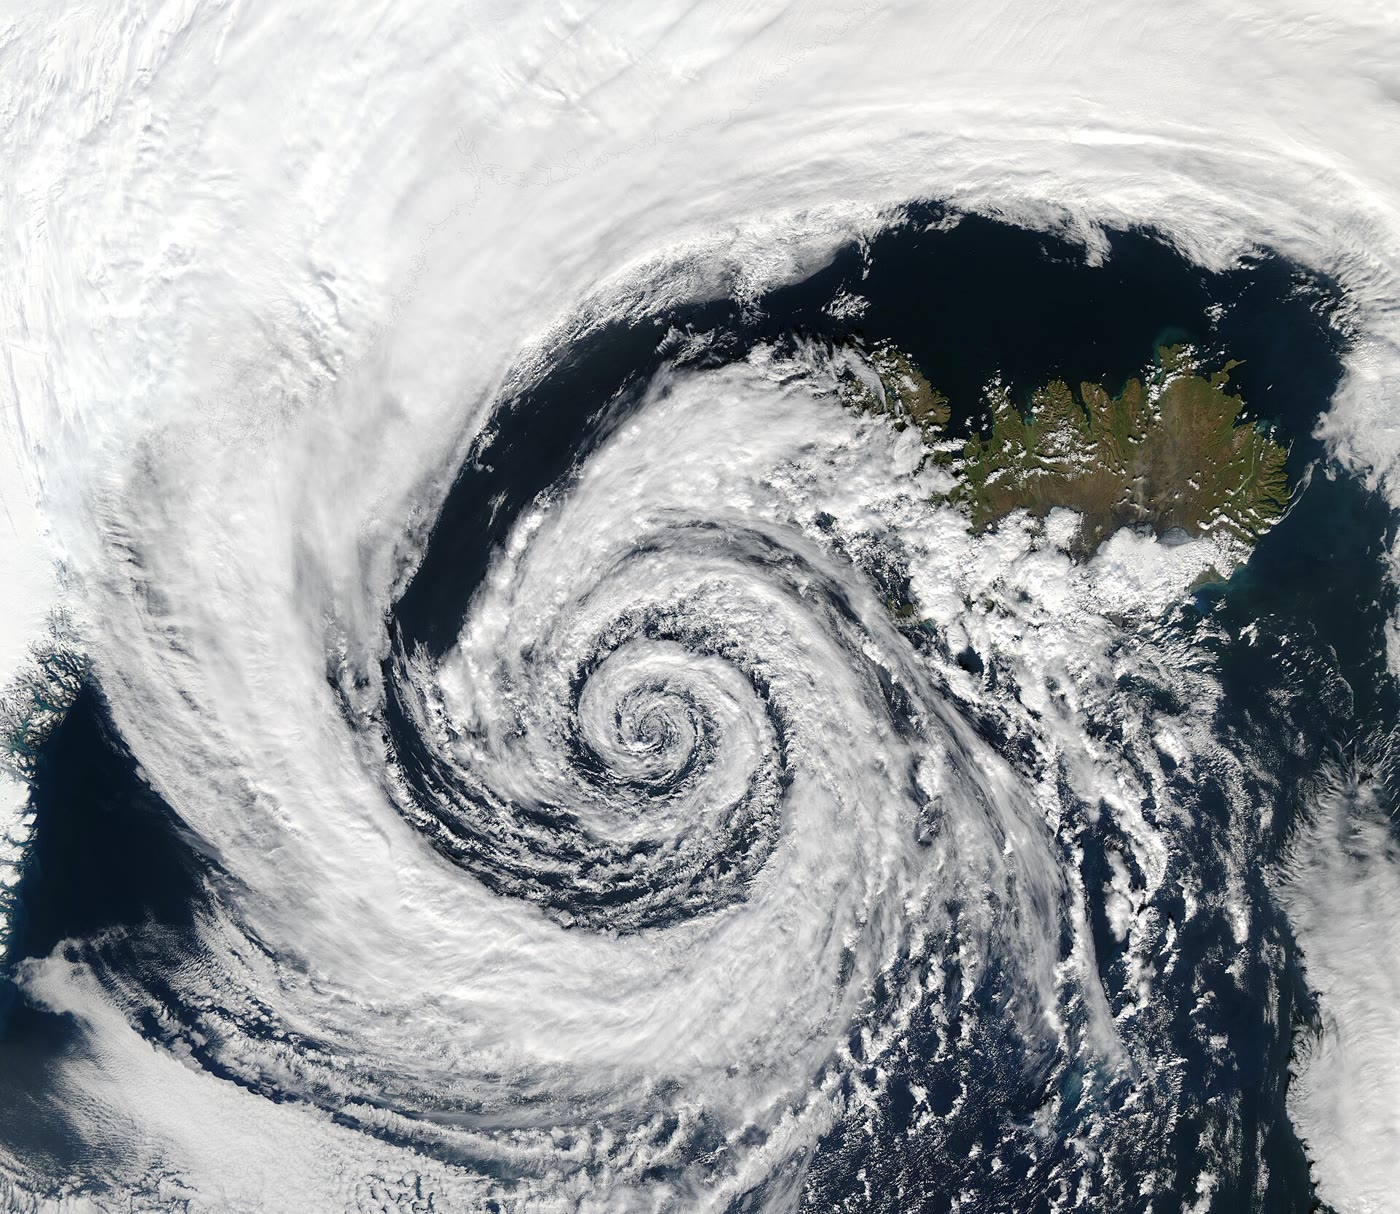
\includegraphics[width=0.58\linewidth]{images/book4/b2-22-iceland-low.jpg}
\par\smallskip{\small 2003 年 9 月 4 日，冰岛西南海岸外的一个深低压，
由 NASA Aqua 卫星的 MODIS 仪器观测：云带螺旋汇入中心。（NASA
Goddard Space Flight Center, MODIS Rapid Response Team, Jacques Descloitres，公有领域，经由
维基共享资源。）}
\end{omfigure}

\section{急流与罗斯贝波}\label{sec:b2:weather-systems:rossby}

气旋并非随机分布。极地急流是极锋之上西风带的快速核心，
它随中纬度高压与低压的位置和移动而变化；它沿其急流段速度最快，
急流段即风速峰值所在的区段，
并且它不绕极地成一个环，而是蜿蜒曲折。
% ledger: nws4:polar-front, nws4:jet-streak

\begin{definition}[罗斯贝波；高空槽与高空脊]\label{def:b2:weather-systems:rossby}
称\emph{罗斯贝波}\index{罗斯贝波}为对流层上部西风气流中的一种波动，
由一系列长达数千千米、南北振幅较大的槽与脊组成。
称\emph{高空槽}\index{高空槽}为这种波动中相对低压的狭长区域，
此处气流向赤道弯曲；称
\emph{高空脊}\index{高空脊}为相对高压的狭长区域，
此处气流向极地弯曲。
\end{definition}
% ledger: nws4:rossby

\omterm{def:b2:weather-systems:rossby}{罗斯贝波}之所以存在，是因为科里奥利参数向极地方向增大。被推向极地的空气
所处的 $f$ 更大，在保持绝对涡度守恒的情况下转向赤道；空气
被推向赤道则转向极地。$f$ 向北增长的速率，
$\beta = \mathrm{d}f/\mathrm{d}y = 2\Omega\cos\varphi/a$，其中 $a$ 为地球半径，决定
它们的速度。本科三年级分册由涡度守恒导出，
波长为 $\lambda$ 的波在均匀西风 $U$ 中的相速度：
\[
  c = U - \frac{\beta}{k^2}, \qquad k = \frac{2\pi}{\lambda} .
\]
此处在本阶段不加证明地承认。相对于空气，每个\omterm{def:b2:weather-systems:rossby}{罗斯贝波}都向西移动，
且波越长，向西移动越快；风则把它向东输送。短波几乎随风速向东移动，
长波则缓慢漂移、停滞，甚至向西移动。
% ledger: earth:Trot, earth:Rmean

\begin{example}[北纬 45° 处的三个波]\label{ex:b2:weather-systems:rossby}
取 $\Omega = \qty{7.292e-5}{s^{-1}}$（恒星日为 \qty{23.9345}{h}），$a =
\qty{6371}{km}$，在北纬 \ang{45} 处 $\beta = \qty{1.62e-11}{m^{-1}.s^{-1}}$。在
风速为 \qty{15}{m/s} 的西风中，波长为 \qty{4000}{km} 的波有 $\beta/k^2 = \qty{6.6}{m/s}$，并以
\qty{8.4}{m/s} 向东移动；波长为 \qty{6000}{km} 的波有 $\beta/k^2 = \qty{14.8}{m/s}$，几乎不动，速度为
\qty{0.2}{m/s}；波长为 \qty{8000}{km} 的波以 \qty{11.2}{m/s} 向西移动。
\end{example}
% ledger: earth:Trot, earth:Rmean

长波的槽移动缓慢、持续时间长；穿行其中的
短波槽在其东侧诱发上升气流，
此处地面气压下降，低压于是形成。轴线由东南指向西北的槽，
往往预示着一个正在发展或增强的系统。
% ledger: nws4:rossby

\begin{omfigure}
\centering
\begin{tikzpicture}[font=\scriptsize, >=Stealth]
\foreach \lat/\pa in {30/-72, 45/-72, 60/-108} {
  \pgfmathsetmacro{\r}{6.0*tan((90-\lat)/2)}
  \draw[black!25] (0,0) circle (\r);
  \node[black!50, fill=white, inner sep=1pt] at (\pa:\r) {北纬\ang{\lat}};
}
\fill (0,0) circle (0.6mm);
\node[anchor=north, black!60] at (0,-0.08) {北极};
\draw[ocBlue, very thick, smooth, samples=241, domain=0:360]
  plot ({6.0*tan((90-(47+11*cos(5*\x)))/2)*cos(\x)}, {6.0*tan((90-(47+11*cos(5*\x)))/2)*sin(\x)});
\foreach \a in {18, 90, 162, 234, 306} {
  \pgfmathsetmacro{\ra}{6.0*tan((90-(47+11*cos(5*\a)))/2)}
  \pgfmathsetmacro{\rb}{6.0*tan((90-(47+11*cos(5*(\a+2))))/2)}
  \draw[ocBlue, very thick, -{Stealth[length=2.6mm]}] (\a:\ra) -- (\a+2:\rb);
}
\pgfmathsetmacro{\rt}{6.0*tan((90-36)/2)}
\node[anchor=216, ocRed!80!black, inner sep=2pt] at (36:\rt) {槽};
\node[anchor=0, ocRed!80!black, inner sep=2pt] at (180:\rt) {槽};
\pgfmathsetmacro{\rr}{6.0*tan((90-58)/2)}
\node[anchor=72, ocRed!80!black, inner sep=3pt] at (72:\rr) {脊};
\end{tikzpicture}
\par\smallskip{\small 从北极上方俯视的急流中的\omterm{def:b2:weather-systems:rossby}{罗斯贝波}（示意）：
半球周围有五个波动，槽伸向赤道，脊伸向
极地。急流向东流动，从北极上方俯视为逆时针方向（箭头）。纬圈
按极射赤面投影地图的方式绘制。}
\end{omfigure}
% ledger: nws4:rossby

有时，这一形势会完全停止移动。

\begin{definition}[大气阻塞]\label{def:b2:weather-systems:blocking}
\emph{大气阻塞}\index{大气阻塞}是一种大范围、持续且几乎静止的高压系统，
有时与低压相伴，它打断了急流正常的向东流动。
大多数阻塞的探测方法都要求其持续至少
五天。
\end{definition}
% ledger: wang26:blocking

阻塞使急流和气旋绕其而行，并使同一地区连续数日维持相同的天气：
阻塞给中纬度地区带来热浪、干旱、野火、寒潮和洪水。
2021 年 6 月下旬至 7 月初，一次强烈的阻塞导致北美洲太平洋西北地区出现热浪，
造成一千多人死亡。阻塞背后的物理过程仍未被充分理解，
数值模式难以再现阻塞的
出现频率及其持续时间。
% ledger: wang26:blocking, wang26:gaps

\section{热带气旋}\label{sec:b2:weather-systems:tropical}

热带气旋没有\omterm{def:b2:weather-systems:fronts}{锋面}，也没有可供其汲取的温度对比。它们的能量
来自温暖的海洋，经由其所蒸发水体的潜热，正如\cref{ch:b2:atmospheric-thermodynamics}
中所测定的那样。有利于其形成的条件有六项：海水温度至少为 \qty{26.5}{\celsius}，
且深度约为 \qty{50}{m}；大气随高度降温足够快，
从而对湿对流不稳定；对流层中部湿度较大，位于 \qty{5}{km} 附近；
离赤道至少约 \qty{500}{km}，使科里奥利力能够维持低压的平衡；
近地面已有扰动；从地面到对流层上部，垂直风切变较弱，低于约
\qty{10}{m/s}。这些条件是必要的，但并不充分：
许多满足这些条件的扰动从未发展成气旋。
% ledger: aoml:tc-genesis

热带气旋一旦形成，便是一台热机。空气在海面上方向内螺旋汇聚，
温度几乎恒定，并从海洋中获取热量和水汽；在眼墙中，空气绝热上升；
在靠近对流层顶的流出层中，空气以辐射方式散热，
此时温度低且几乎恒定；远离中心处，空气再次下沉，
完成一个与卡诺循环相似的循环。循环所做的功驱动风
克服海面摩擦而运动。
% ledger: gilford21:pi

\begin{omfigure}
\centering
\begin{tikzpicture}[font=\scriptsize, >=Stealth, x=1cm, y=1cm]
% sea and axis
\fill[ocBlue!12] (0,-0.35) rectangle (12.5,0);
\draw[thick, ocBlue!70!black] (0,0) -- (12.5,0);
\node[anchor=north west, ocBlue!70!black] at (8.6,-0.02) {暖海，$T_s$};
\draw[dashed, black!50] (0,-0.35) -- (0,4.9);
\node[anchor=south, black!60] at (0,4.9) {中心};
% eyewall cloud and outflow cloud
\fill[black!14, draw=black!40] (0.9,0.25) .. controls (0.7,1.8) and (0.75,3.3) .. (0.95,4.2)
  .. controls (3.5,4.55) and (7.0,4.45) .. (9.5,4.2) .. controls (7.0,3.9) and (3.6,3.85)
  .. (2.1,3.7) .. controls (1.95,2.6) and (1.9,1.4) .. (2.0,0.25) -- cycle;
\node[black!60] at (0.45,2.0) [rotate=90] {风暴眼};
\draw[black!50] (1.9,1.1) -- (2.45,1.1) node[anchor=west, black!70] {眼墙云};
% the cycle
\draw[->, very thick, ocRed] (11.4,0.3) -- (2.3,0.3);
\draw[->, very thick, ocRed] (1.45,0.45) .. controls (1.4,1.6) and (1.45,3.0) .. (1.75,4.0);
\draw[->, very thick, ocBlue] (2.2,4.25) -- (11.2,4.25);
\draw[->, very thick, ocBlue] (11.6,4.05) .. controls (11.75,2.8) and (11.75,1.5) .. (11.6,0.45);
\fill (11.6,0.3) circle (0.7mm) node[right=2pt] {A};
\fill (1.45,0.3) circle (0.7mm) node[left=2pt] {B};
\fill (1.8,4.25) circle (0.7mm) node[above left=1pt] {C};
\fill (11.6,4.25) circle (0.7mm) node[above right=1pt] {D};
\node[anchor=south, align=center] at (6.5,0.35) {A$\to$B：海面上方的流入，温度约为 $T_s$，
  吸收热量和水汽};
\node[anchor=west, align=left] at (2.25,2.3) {B$\to$C：在眼墙中上升，\\
  不与外界交换热量（湿绝热线）};
\node[anchor=south, align=center] at (6.5,4.62) {C$\to$D：流出层靠近对流层顶，温度约为
  $T_o$，以辐射方式散热};
\node[anchor=east, align=right] at (11.45,2.3) {D$\to$A：下沉 \\远离中心处};
\end{tikzpicture}
\par\smallskip{\small 热带气旋的热机，自中心向外的竖直剖面
（示意图，未按比例）：热量在海面温度下被吸收
（A$\to$B），并在低得多的流出层温度下放出（C$\to$D），如
卡诺循环一样。}
\end{omfigure}
% ledger: gilford21:pi

\begin{proposition}[潜在强度]\label{prop:b2:weather-systems:pi}
\index{潜在强度}
热带气旋的\emph{\omterm{prop:b2:weather-systems:pi}{潜在强度}}，即其周围海洋与大气所能维持的
近地面最大风速，近似由下式给出：
\[
  V_{\max}^2 = \frac{C_k}{C_D}\,\frac{T_s - T_o}{T_o}\,\bigl(h_o^* - h^*\bigr),
\]
其中 $T_s$ 为海面温度，$T_o$ 为流出层温度，$C_k/C_D$
为海气之间焓与动量交换系数之比，
通常取为 0.9，$h_o^* - h^*$ 为海面处饱和时的 $c_pT + gz + Lq$ 相对于
边界层上方空气中其饱和值的超出量（在本阶段不加证明地承认）。
\end{proposition}
% ledger: gilford21:pi

分式 $(T_s - T_o)/T_o$ 并不是物理教材中的卡诺效率 $(T_s - T_o)/T_s$：
它大出的倍数为 $T_s/T_o$，原因在于耗散掉功的摩擦力加热了
海面附近流入的空气，这部分热量又被热机利用。最后一
因子代表燃料。在热带大气中，其温度沿其边界层空气的\omterm{def:b2:atmospheric-thermodynamics:moist-adiabat}{湿绝热线}变化，
$h^*$ 即该空气中 $c_pT + gz + Lq$ 的值，$h_o^* - h^*$
度量海面上方空气与海温下饱和状态相差多远：
\[
  h_o^* - h^* \approx c_p\,(T_s - T_a) + L\,(q_s^* - q_a),
\]
其中 $T_a$ 与 $q_a$ 分别为近地面空气的温度与\omterm{def:b2:atmospheric-thermodynamics:moist-air}{比湿}，
$q_s^*$ 为海面温度下的饱和\omterm{def:b2:atmospheric-thermodynamics:moist-air}{比湿}。
% ledger: gilford21:pi

\begin{example}[潜在强度示例]\label{ex:b2:weather-systems:pi}
在 \qty{29}{\celsius} 的海面上，\qty{1015}{hPa} 的空气温度为 \qty{28}{\celsius}，
相对湿度为 \qty{80}{\percent}，流出层温度为 \qty{200}{K}，这是温暖热带海洋上的典型年平均值。
由\cref{prop:b2:atmospheric-thermodynamics:es,prop:b2:atmospheric-thermodynamics:humidity}，
$e_s(\qty{29}{\celsius}) = \qty{41.0}{hPa}$，因此 $q_s^* = \qty{25.5}{g/kg}$；空气
的 $e = 0.8 \times \qty{38.7}{hPa}$，则 $q_a = \qty{19.2}{g/kg}$。于是 $h_o^* - h^* = 1004.5 \times
1 + 2.501 \times 10^6 \times 0.0063 = \qty{16.8}{kJ/kg}$，因子 $(T_s - T_o)/T_o$ 为
$(302.15 - 200)/200 = 0.511$，且 $V_{\max} = \sqrt{0.9 \times 0.511 \times 16\,800} =
\qty{88}{m/s}$。
\end{example}
% ledger: gilford21:pi

最强的风暴接近这些数值：萨菲尔–辛普森等级的最高一级，
即 5 级，起始风速为 \qty{70}{m/s}，近期已有五场风暴超过 \qty{86}{m/s}。
多数风暴很少达到其\omterm{prop:b2:weather-systems:pi}{潜在强度}：实际风暴很少处于理论所假设的
稳态，理论中忽略了垂直风切变、被卷入风暴的干空气，以及
其周围空气的下沉运动，这些因素都会削弱风暴。
% ledger: wk24:scale, gilford21:limits, aoml:tc-weaken

\begin{omfigure}
\centering
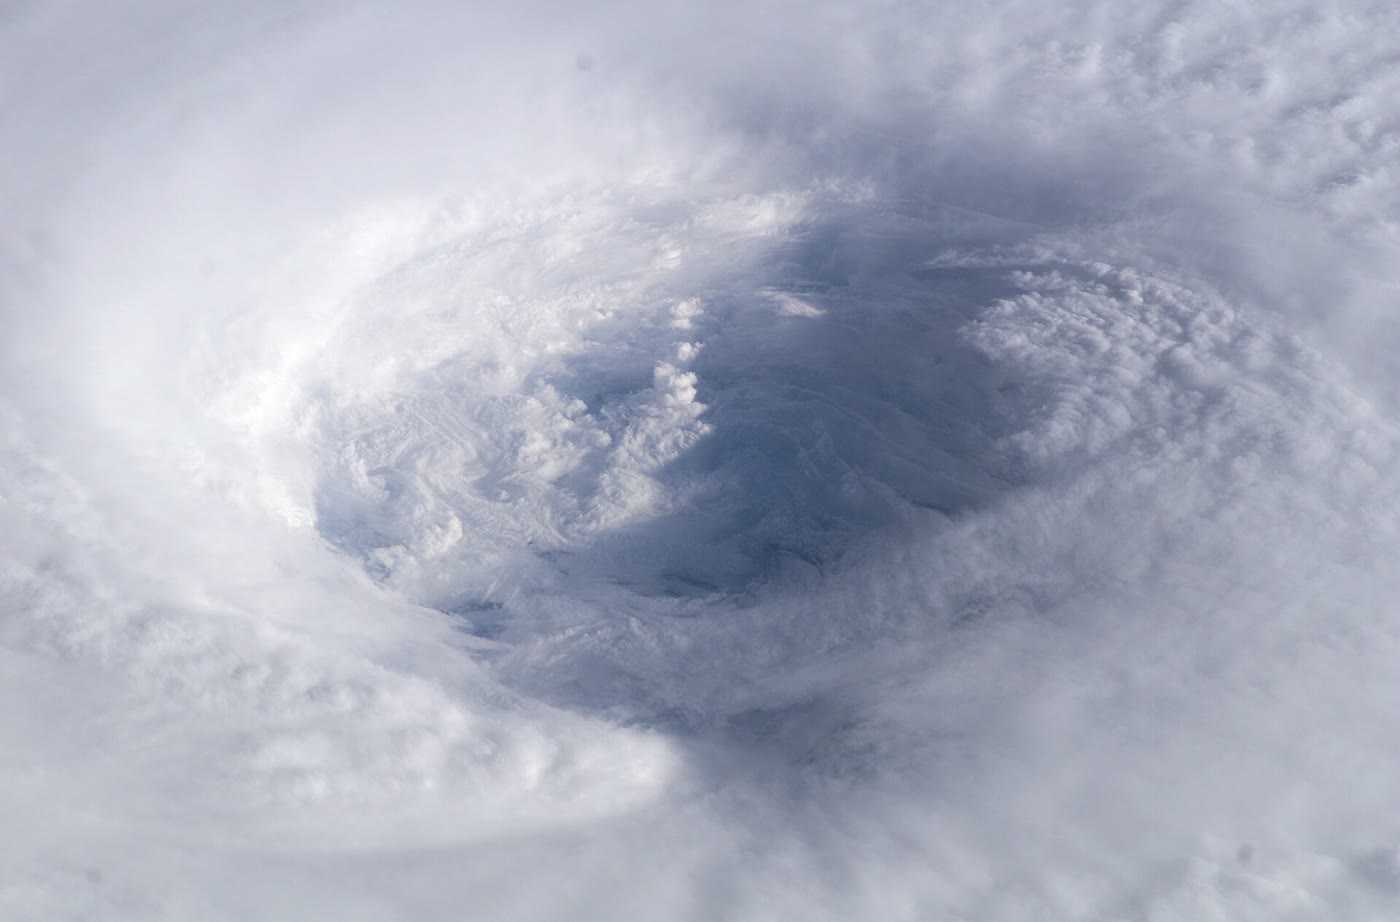
\includegraphics[width=0.62\linewidth]{images/book4/b2-22-isabel-eye.jpg}
\par\smallskip{\small 飓风“伊莎贝尔”的风暴眼，2003 年 9 月 13 日，自
国际空间站拍摄：眼墙如体育场看台般向下延伸，直至风暴眼中的低云。
（NASA 宇航员 Ed Lu，公有领域，经维基共享资源。）}
\end{omfigure}

\section{数值天气预报}\label{sec:b2:weather-systems:nwp}

\begin{definition}[数值天气预报；资料同化；集合预报；可预报性极限]\label{def:b2:weather-systems:nwp}
\emph{数值天气预报}\index{数值天气预报}是借助计算机进行的预报：
即由描述大气运动、能量与水分的方程，
从其观测状态出发，沿时间向前积分。\emph{资料同化}\index{资料同化}
将最新观测与较早观测给出的短期预报相结合，
以得到当前状态的最优估计（即分析场）；
预报由此开始。\emph{集合预报}\index{集合预报}是一组预报，
由略有不同的初始状态及略有不同版本的模式运行得到，
以显示可能出现的天气范围及其可能性。\emph{可预报性
极限}\index{可预报性极限}是指这样一个时间：超过该时间后，天气状态的预报
已不优于依据气候作出的猜测，因为初始状态的误差
已增长到与大气任意两种状态之间的差异同样大。
\end{definition}
% ledger: nws4:nwp, ecmwf4:da, ecmwf4:ens-fs, krish19:predictability

第一次数值预报于 1950 年在 ENIAC 上完成，ENIAC 是最早的电子计算机之一。
如今的全球模式将大气划分为边长若干千米的网格单元，
并从分析场出发开始积分。分析场融合了来自气象站、飞机、探空仪、船舶、浮标的观测，
以及最重要的卫星观测；卫星对全球预报技巧的贡献最大。
某大型预报中心的\omterm{def:b2:weather-systems:nwp}{集合预报}
包含 51 个成员，即 1 个对照运行与 50 个扰动成员，分辨率约为 \qty{9}{km}，
每天运行两次，向前预报 15 天。
% ledger: krish19:predictability, ecmwf4:da, ecmwf4:ens

既然可以从最佳分析场出发，为何还要对预报进行扰动？
原因在于大气具有混沌性，对初始状态十分敏感。
1963 年发表的一个三变量系统在最小尺度上展示了这一点。

\begin{proposition}[洛伦茨系统]\label{prop:b2:weather-systems:lorenz}
考虑如下系统
\[
  \dot x = \sigma(y - x), \qquad \dot y = x(r - z) - y, \qquad \dot z = xy - bz,
\]
其中 $\sigma = 10$、$r = 28$ 与 $b = 8/3$，该系统具有下列性质。
\begin{enumerate}
  \item 其不动点为原点及 $C_\pm = \bigl(\pm\sqrt{b(r - 1)}, \pm\sqrt{b(r - 1)},
        r - 1\bigr) = (\pm 8.49, \pm 8.49, 27)$。
  \item 相空间中每一体积按 $\mathrm{e}^{-(\sigma + 1 + b)t}$ 收缩：其
        轨迹最终落在零体积的集合上，该集合即吸引子。
  \item 在吸引子上，起始相距很小距离 $\delta_0$ 的两条轨迹，
        平均而言按 $\delta(t) \approx \delta_0\,\mathrm{e}^{\lambda t}$ 分离，其中 $\lambda =
        0.906$，直至 $\delta$ 达到吸引子的大小（由计算得到，在本阶段不加证明地承认）。小
        误差每 $\ln 2/\lambda = 0.77$ 个时间单位翻一番。
\end{enumerate}
\end{proposition}
% ledger: nolitia22:lorenz

\begin{proof}[1 与 2 的证明]
在不动点处，由第一个方程得 $y = x$；第三个方程给出 $z = x^2/b$；第二个方程
化为 $x(r - 1 - x^2/b) = 0$，故 $x = 0$ 或 $x^2 = b(r - 1) = 72$。该
向量场的散度为 $\partial_x\dot x + \partial_y\dot y + \partial_z\dot z = -\sigma - 1 - b$，
为常数。由散度定理，流动所携带的体积 $V$ 满足 $\dot V =
-(\sigma + 1 + b)V$。
\end{proof}

图形说明了该命题的含义。起始相距 \num{e-5} 的两次运行
在约十五个时间单位内彼此跟随，随后永久分开：二者各自看起来仍像该系统的一条合理轨迹，
但已不再是同一条轨迹。对 200 对运行取平均，
这些运行起始相距 \num{e-8}，间距以速率 $\lambda$ 呈指数增长，
在对数坐标下为一条直线，直至在吸引子大小处饱和。无论初始误差多大，
它终将达到这一大小：较小的初始误差只会将这一时刻推迟，
初始误差每缩小十倍，推迟 $\ln 10/\lambda = 2.5$ 个时间单位。
% ledger: nolitia22:lorenz

\begin{omfigure}
\centering
% figdata/bachelor-2/weather.py parts traj, butterfly
\begin{tikzpicture}
\begin{groupplot}[group style={group size=2 by 1, horizontal sep=1.5cm},
  tick label style={font=\scriptsize}, label style={font=\small}]
\nextgroupplot[width=0.58\linewidth, height=5.0cm, xmin=0, xmax=30, ymin=-22, ymax=22,
  xlabel={时间}, ylabel={$x$}, legend style={font=\scriptsize, at={(0.5,1.02)},
  anchor=south, draw=none, legend columns=2, /tikz/every even column/.append style={column
  sep=0.4cm}}, legend cell align=left]
\addplot[ocBlue, thin] table[x=t, y=x1] {figdata/out/bachelor-2-weather-traj.dat};
\addlegendentry{运行 1}
\addplot[ocRed, thin, densely dashed] table[x=t, y=x2] {figdata/out/bachelor-2-weather-traj.dat};
\addlegendentry{运行 2，起始相距 \num{e-5}}
\nextgroupplot[width=0.4\linewidth, height=5.0cm, xmin=-22, xmax=22, ymin=0, ymax=52,
  xlabel={$x$}, ylabel={$z$}]
\addplot[black!70, very thin] table[x=x, y=z] {figdata/out/bachelor-2-weather-butterfly.dat};
\addplot[only marks, mark=*, mark size=1.3pt, ocRed] coordinates {(8.485,27) (-8.485,27)};
\end{groupplot}
\end{tikzpicture}
\par\smallskip{\small 洛伦茨系统（$\sigma = 10$，$r = 28$，$b = 8/3$），用
龙格–库塔方法积分，时间步长为 0.01。左图：两次运行起始时在 $x$ 方向相距 \num{e-5}，
均位于吸引子上。右图：一次运行持续 40 个时间单位，沿 $y$ 方向观察，
并标出不动点 $C_\pm$（红色）。}
\end{omfigure}
% ledger: nolitia22:lorenz

\begin{omfigure}
\centering
% figdata/bachelor-2/weather.py part growth
\begin{tikzpicture}
\begin{axis}[width=0.72\linewidth, height=5.6cm, xmin=0, xmax=30, ymode=log, ymin=1e-9,
  ymax=1e3, ytick={1e-9,1e-7,1e-5,1e-3,1e-1,1e1,1e3}, xlabel={时间}, ylabel={两次运行之间的距离}, tick label style={font=\scriptsize},
  label style={font=\small}, legend style={font=\scriptsize, at={(0.02,0.98)}, anchor=north west,
  draw=none, fill=none}, legend cell align=left, unbounded coords=discard, grid=major,
  grid style={black!8}]
\addplot[ocBlue, line width=1.6pt, opacity=0.55] table[x=t, y expr=10^\thisrow{log10d}]
  {figdata/out/bachelor-2-weather-growth.dat};
\addlegendentry{200 对运行的几何平均}
\addplot[black, densely dashed, thin] table[x=t, y expr=10^\thisrow{fit}]
  {figdata/out/bachelor-2-weather-growth.dat};
\addlegendentry{拟合指数，$t = 2$ 至 16}
\end{axis}
\end{tikzpicture}
\par\smallskip{\small 洛伦茨系统各对运行之间距离的增长，起始相距
\num{e-8}。拟合直线每 2.57 个时间单位增大十倍，增长率为 0.897；
最大李雅普诺夫指数由单对运行、经 2000 个时间单位的重归一化计算得到，为
0.909，与已发表的 0.906 相比。增长止于吸引子的大小。}
\end{omfigure}
% ledger: nolitia22:lorenz

大气的行为与此相同，只是变量多得多，误差
在不同尺度上以不同速率增长。根据 1980 年代的预报，人们发现小误差
约在 2.4 天内翻一番，而天气状态的可靠预报大约只能做到十天左右。
在假定模式完美的前提下，缩小当前初始状态不确定度的实验表明，
完美的初始条件只能再增加四至五天，
而将不确定度减小 90\% 即可获得几乎全部的收益：误差越小，增长越快，
其原因在于对流中潜热的释放，发生在预报分辨率所无法分辨的更小尺度上。
中纬度的\omterm{def:b2:weather-systems:nwp}{可预报性极限}约为两周。预报
的时效每十年约增加一天，这得益于更好的观测、\omterm{def:b2:weather-systems:nwp}{资料同化}与模式，
使预报逐渐逼近该极限，却无法越过它。
% ledger: krish19:predictability, selz22:limit, bauer:day-per-decade

\omterm{def:b2:weather-systems:nwp}{集合预报}将这一点变成了工具。各成员从彼此之间的差异约等于分析本身不确定度的分析场出发；
当各成员彼此接近时，预报就很明确；当它们发散时，预报必须予以说明，并给出概率。
若预报宣称某事件将以 \qty{70}{\percent} 的概率发生，
且在 \qty{70}{\percent} 的情形中该事件确实发生，
则称该预报是可靠的。
% ledger: ecmwf4:ens-fs

\begin{inthelab}[一个预报中心的一天]
\begin{minipage}[t]{0.54\linewidth}\vspace{0pt}
一个全球预报中心每天两轮工作，分别对应 00 UTC 和 12 UTC 两个时次。
每一时次前后有效的观测多达数百万条，来自卫星、探空仪、飞机、船舶、浮标和气象站；
\omterm{def:b2:weather-systems:nwp}{资料同化}将这些观测与前一次短期预报融合，得到分析场。
模式与\omterm{def:b2:weather-systems:nwp}{集合预报}都从该分析场出发，预报结果送达用户，
通常在数小时后，此时超级计算机已完成未来 15 天的计算。
预报员随后比对各个预报结果，
对照最新观测和卫星图像加以检验，追踪气旋与锋，
并将\omterm{def:b2:weather-systems:nwp}{集合预报}的概率转化为预警和预报。
\end{minipage}\hfill
\begin{minipage}[t]{0.42\linewidth}\vspace{0pt}
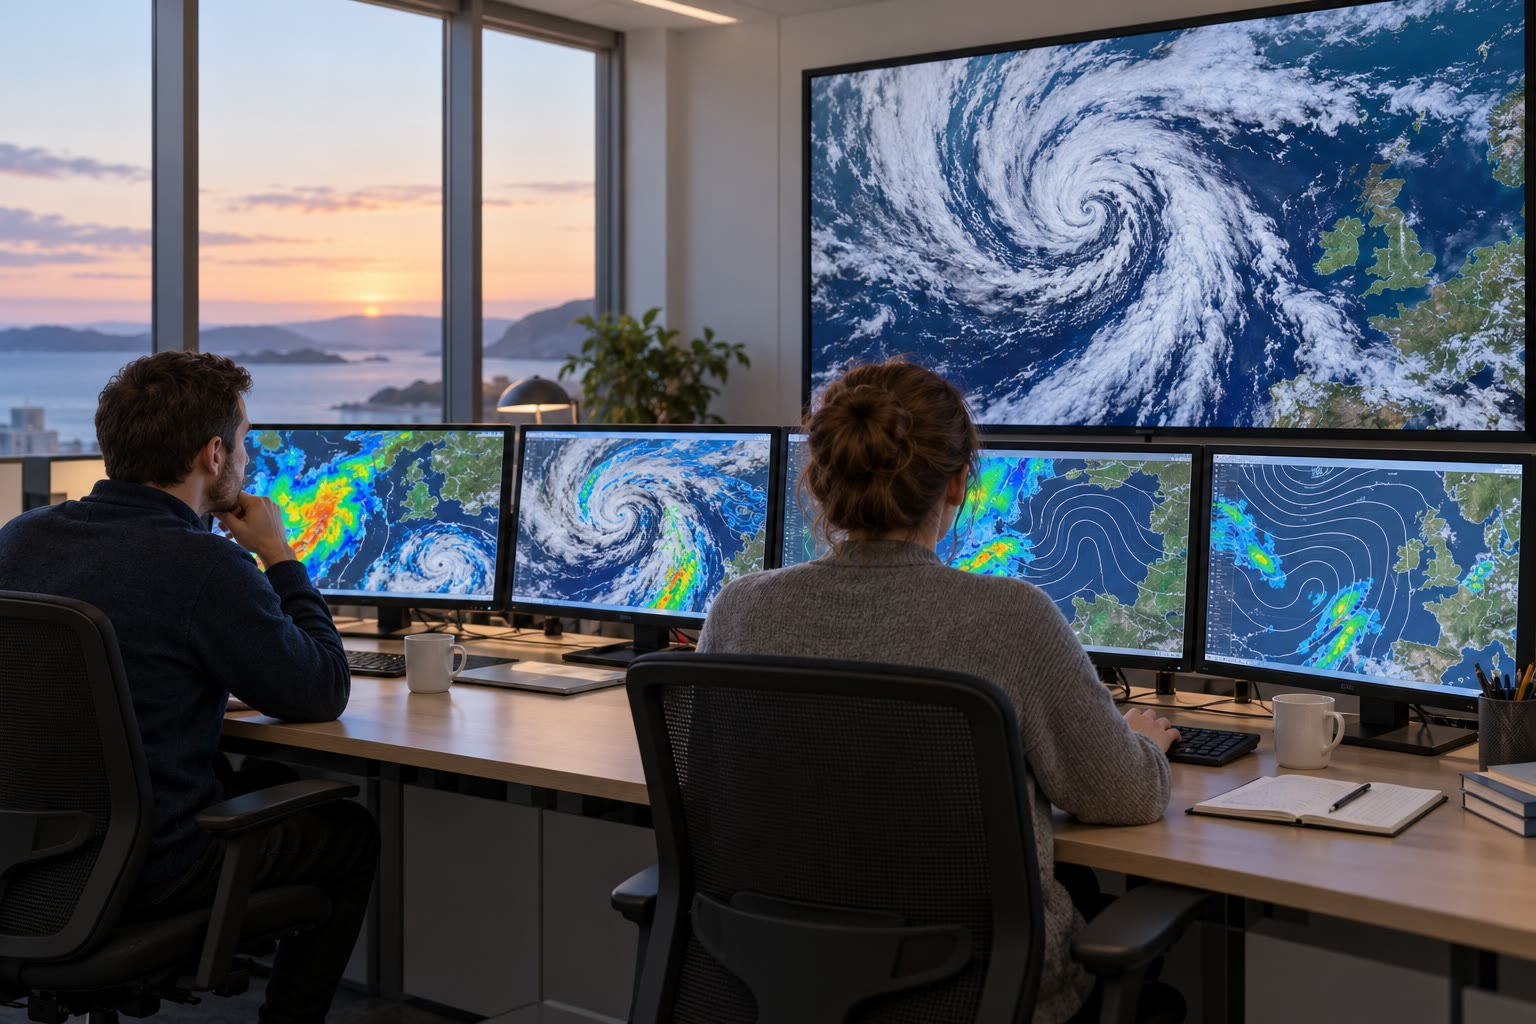
\includegraphics[width=\linewidth]{images/book4/ai/b2-forecast-office.jpg}

{\scriptsize 预报员在卫星图像和模式图表前工作
（AI 生成的插图）。}
\end{minipage}
% ledger: ecmwf4:ens, ecmwf4:da, mo:how-forecasts
\end{inthelab}

\section*{练习}\label{sec:b2:weather-systems:exercises}

除非另有说明，练习数据取为：$\Omega = \qty{7.292e-5}{s^{-1}}$，$a =
\qty{6371}{km}$, $g = \qty{9.81}{m.s^{-2}}$, $c_p = \qty{1004.5}{J.kg^{-1}.K^{-1}}$, $L =
\qty{2.501e6}{J/kg}$，以及
\cref{ch:b2:atmospheric-thermodynamics}练习中的饱和\omterm{def:b2:atmospheric-thermodynamics:moist-air}{水汽压}。
% ledger: earth:Trot, earth:Rmean

\begin{exercise}[$\star$]\label{exo:b2:weather-systems:1}
在北纬 \ang{50}，一条冷锋将 \qty{275}{K} 的空气与 \qty{281}{K} 的空气分开，
沿锋的风速变化 \qty{15}{m/s}。(a) 计算 $f$。(b) 计算\omterm{def:b2:weather-systems:fronts}{锋面}的坡度，
以 1 比 $N$ 的形式表示。(c) \omterm{def:b2:weather-systems:fronts}{锋面}在地面上位于锋后多远处达到
\qty{1}{km} 的高度？(d) 若在相同的风切变下温度对比加倍，
坡度会如何变化？
\end{exercise}

\begin{exercise}[$\star$]\label{exo:b2:weather-systems:2}
暖\omterm{def:b2:weather-systems:fronts}{锋面}以 1 比 150 的坡度上升，并以 \qty{25}{km/h} 的速度移动。(a) 当\omterm{def:b2:weather-systems:fronts}{锋面}高度为 \qty{6}{km} 时，
它在地面上位于锋前多远处？(b) 一名观测者在该处看到高层云在\omterm{def:b2:weather-systems:fronts}{锋面}上形成。
问\omterm{def:b2:weather-systems:fronts}{锋面}再经过多久到达该观测者处？(c) 描述
观测者在此期间看到的云系变化顺序。
\end{exercise}
% ledger: ucar:warm-front

\begin{exercise}[$\star$]\label{exo:b2:weather-systems:3}
在北半球的一张图上：(a) 一条蓝色三角形位于其东南侧的线，自一个低压向西南延伸；
(b) 一条红色半圆位于其北侧的线，自同一低压向东延伸；(c) 一条同时带有两种符号的紫色线，
从另一个低压延伸至另外两条锋开始的点；
(d) 一条线在南侧为蓝色三角形、北侧为红色半圆交替出现。
逐一说明各条锋的名称，指出冷空气所在位置以及每条锋的移动方向。
\end{exercise}
% ledger: ucar4:stationary-occluded, nws4:occluded

\begin{exercise}[$\star$]\label{exo:b2:weather-systems:4}
在北纬 \ang{45}、风速为 \qty{12}{m/s} 的西风中：(a) 计算 $\beta$。(b) 计算
波长为 \qty{4000}{km} 和 \qty{8000}{km} 的波的相速度。(c) 每个波向哪个方向移动，
一天内移动多远？
\end{exercise}

\begin{exercise}[$\star\star$]\label{exo:b2:weather-systems:5}
(a) 证明在西风 $U$ 中，当 $\lambda = 2\pi\sqrt{U/\beta}$ 时，\omterm{def:b2:weather-systems:rossby}{罗斯贝波}静止不动。
(b) 在北纬 \ang{45}，取 $U = \qty{12}{m/s}$，计算该波长。(c) 绕纬圈能容纳
多少个这样的波？(d) 为什么更强的西风有利于出现数量更少、波长更长的驻波？
\end{exercise}

\begin{exercise}[$\star\star$]\label{exo:b2:weather-systems:6}
对于洛伦茨系统：(a) 通过计算该点处的三个导数，验证 $C_+$ 是不动点。
(b) 在一个时间单位内，相空间中的小体积会缩小为原来的几分之几？(c) 为什么
这并不妨碍两条相近轨迹相互分离？
\end{exercise}

\begin{exercise}[$\star\star$]\label{exo:b2:weather-systems:7}
取洛伦茨系统中 $\lambda = 0.906$，吸引子的尺度为 10。(a) 计算小误差的倍增时间。
(b) 误差为 \num{e-8} 时，需要多长时间才能增长到吸引子的尺度？
(c) 初始误差小一千倍时，这一时刻推迟多少？
该推迟时间占 (b) 中所求时间的几分之几？
\end{exercise}
% ledger: nolitia22:lorenz

\begin{exercise}[$\star\star$]\label{exo:b2:weather-systems:8}
海面温度为 \qty{303}{K}，流出层温度为 \qty{195}{K}；非平衡量为 $h_o^* - h^* =
\qty{15}{kJ/kg}$，且 $C_k/C_D = 0.9$。(a) 计算\omterm{prop:b2:weather-systems:pi}{潜在强度}。(b) 将其与
萨菲尔–辛普森五级的阈值以及近期最强的风暴进行比较。(c) 为什么大多数风暴
达不到该强度？
\end{exercise}
% ledger: gilford21:pi, wk24:scale

\begin{exercise}[$\star\star$]\label{exo:b2:weather-systems:9}
对于\cref{exo:b2:weather-systems:8}中的风暴：(a) 计算工作于海面与流出层之间的卡诺热机的效率。
(b) 计算\cref{prop:b2:weather-systems:pi}中的因子 $(T_s - T_o)/T_o$，
以及两者之比。(c) 解释二者的差异。
\end{exercise}
% ledger: gilford21:pi

\begin{exercise}[$\star\star\star$]\label{exo:b2:weather-systems:10}
(a) 在保留密度精确值的情况下重新推导\cref{prop:b2:weather-systems:slope}，并证明
冷空气必定位于下方。(b) 在北纬 \ang{45}，宽 \qty{50}{km} 的锋区内，沿锋的风速变化
\qty{10}{m/s}。计算该锋区的相对涡度，并与 $f$ 比较。
(c) 该锋区是气旋性的还是反气旋性的？
\end{exercise}

\begin{exercise}[$\star\star\star$]\label{exo:b2:weather-systems:11}
假设预报误差每 2.4 天翻一番，初始误差为 \qty{0.5}{K}，误差达到 \qty{6}{K} 时预报即无用。
(a) 求有用预报的时效极限。(b) 若模式是完美的，初始误差每十年需缩小为原来的几分之几，
才能使预报时效每十年增加一天？(c) 实验发现，初始误差缩小十倍只能增加 4 至 5 天的时效。
由此推得小误差的倍增时间为多少？
这说明小误差是如何增长的？
\end{exercise}
% ledger: krish19:predictability, selz22:limit, bauer:day-per-decade

\begin{exercise}[$\star\star\star$]\label{exo:b2:weather-systems:12}
取 \cref{ex:b2:weather-systems:pi}，将海洋与空气都升温 \qty{1}{K}，
相对湿度与流出温度保持不变。(a) 重新计算 $q_s^*$、$q_a$ 和
非平衡度。(b) 重新计算\omterm{prop:b2:weather-systems:pi}{潜在强度}。(c) 每开尔文它增加百分之几，
以及哪一项贡献最大？
\end{exercise}
% ledger: gilford21:pi

\begin{problem}[{周末问题——能预报多远？}]\label{pb:b2:weather-systems:1}
一张虚构的天气图显示，北纬\ang{50}处一条冷锋正逼近某城镇，并伴有一列\omterm{def:b2:weather-systems:rossby}{罗斯贝波}，
位于其上方急流中。本题先讨论\omterm{def:b2:weather-systems:fronts}{锋面}，再讨论波动，然后问其中任一部分能提前多久预报，
请利用练习中的数据。

\medskip\noindent\textbf{第一部分——\omterm{def:b2:weather-systems:fronts}{锋面}。}
06 UTC 时冷锋位于小镇以西 \qty{480}{km}，12 UTC 时位于 \qty{390}{km} 处。锋后
空气温度为 \qty{277}{K}，暖区内为 \qty{285}{K}，沿锋的风速
穿过\omterm{def:b2:weather-systems:fronts}{锋面}变化了 \qty{16}{m/s}。
\begin{enumerate}
  \item 求\omterm{def:b2:weather-systems:fronts}{锋面}的移动速度。
  \item \omterm{def:b2:weather-systems:fronts}{锋面}何时到达小镇？
  \item 计算北纬\ang{50}处的 $f$。
  \item 计算\omterm{def:b2:weather-systems:fronts}{锋面}的坡度。
  \item 求\omterm{def:b2:weather-systems:fronts}{锋面}经过后六小时，它在小镇上方的高度。
  \item 求冷空气到达小镇上方 \qty{1.5}{km} 处所需的时间（自\omterm{def:b2:weather-systems:fronts}{锋面}经过起算）。
  \item \omterm{def:b2:weather-systems:fronts}{锋面}经过时小镇出现什么天气，气压如何变化？
\end{enumerate}

\medskip\noindent\textbf{第二部分——高空的波动。}
在上方急流中，西风为 \qty{20}{m/s}，波长为 \qty{5000}{km}。
\begin{enumerate}[resume]
  \item 计算北纬\ang{50}处的 $\beta$。
  \item 计算 $k$ 及 $\beta/k^2$。
  \item 求该波的相速度。
  \item 一个槽在 24 小时内移动多远？
  \item 求在此风速下静止不动的波长，以及
        环绕北纬\ang{50}一周可容纳多少个此类波。
  \item 相对于\omterm{def:b2:weather-systems:rossby}{高空槽}，地面气旋应在何处加深？
\end{enumerate}

\medskip\noindent\textbf{第三部分——简化大气模型。}
在洛伦茨系统误差增长的图中，拟合直线经过
$t = 4$ 时约 \num{5e-7}，$t = 14$ 时约 \num{3.9e-3}。
\begin{enumerate}[resume]
  \item 由这两个读数计算增长率 $\lambda$。
  \item 计算倍增时间。
  \item 与已发表的指数 0.906 进行比较。
  \item 距离为何在 15 左右停止增长？
  \item 误差小十倍时，要晚多久才能达到同样的大小？
\end{enumerate}

\medskip\noindent\textbf{第四部分——能预报多远？}
取 1980 年代预报中小误差所得的倍增时间 2.4 天，
某一高度温度的初始误差为 \qty{0.1}{\celsius}，且
预报在误差达到 \qty{3}{\celsius} 时即失效。
\begin{enumerate}[resume]
  \item 初始误差到失效误差之间相隔几次倍增？
  \item 这需要多少天？
  \item 将初始误差减半，能多得到多少天的预报？
  \item 若采用此前估计的 5 天倍增时间，得到的预报时限为多少？
  \item 现代实验表明，即使初始误差小十倍，甚至初始状态完全精确，
        也只能多得 4 至 5 天。这为何说明
        第 20 问中的估计偏于乐观？
  \item 综上所述，以天计，该预报能有效提前多少天？
\end{enumerate}
\end{problem}
% ledger: krish19:predictability, selz22:limit, nolitia22:lorenz, ucar:cold-front
